
Many domains of science rely on smooth approximations to real-valued functions over a closed interval. These smooth approximations are regularly used in automotive and aerospace engineering, architecture, mathematics and especially statistics \cite{knott2012interpolating}. While polynomial interpolants or regressors apply broadly, piecewise polynomial functions (splines) are often a good choice because they can approximate globally complex functions while minimizing local complexity of the approximation. It is often the case that the true underlying function or phenomenon being modeled has known properties e.g., convexity, positivity, various levels of continuity, or monotonicity. Given a reasonably large amount of data, it can be impossible to maintain these properties with a single polynomial function.

In general, the maintenance of function properties through interpolation / regression is usually referred to as \textit{shape preserving} \cite{fritsch1980monotone,gregory1985shape}. The specific shapes this work will focus on are monotonicity and multiple levels of continuity for a function. These properties are chiefly important to the approximation of cumulative distribution functions and subsequently the effective generation of random numbers from a specified distribution. 

In statistics especially, the construction of a monotone interpolating spline that is continuous in second derivative is meaningfully useful \cite{ramsay1988monotone}. A function with these properties could approximate random variables to a high level of accuracy with relatively few intervals (with even more accuracy given greater continuity). A continuously twice differentiable approximation to a cumulative distribution function would also produce a corresponding probability density function that is continuously differentiable, which is a property many commonly occurring parametric distributions maintain.


\section{Related Work}

The current state-of-the-art monotone interpolating spline with a mathematical software implementation is piecewise cubic, continuously differentiable, and was first proposed in \citet{fritsch1980monotone} then expanded upon in \citet{carlson1985monotone}. Let $\pi: a = x_1 < x_2 < \cdots < x_n = b$ be a partition of the interval $[a,b]$. Let $\{f(x_i) : i = 1,2,\ldots,n\}$ be a given set of data values at the partition points for a monotone function $f$, meaning $f(x_i) \leq f(x_{i+1})$ for $i = 1, \ldots, n-1$ or $f(x_i) \geq f(x_{i+1})$ for $i = 1, \ldots, n-1$. Let $\hat f$ be a piecewise cubic spline defined in each sub-interval $I_i = [x_i, x_{i+1}]$ by

\begin{align*}
h_i =& \ x_{i+1} - x_{i} \\
u(t) =& \ 3t^2 - 2t^3 \\
p(t) =& \ t^3 - t^2 \\
\hat f(x) =& \ f(x_i)\ u\big((x_{i+1} - x) / h_i\big) + f(x_{i+1})\ u\big((x - x_i) / h_i\big) \\
& - \hat f^{\ \prime}(x_i)\ p\big((x_{i+1}-x)/h_i\big) + \hat f^{\ \prime}(x_{i+1})\ p\big((x-x_i)/h_i \big).
\end{align*}

Notice that it is up to the user to choose values for $\hat f^{\ \prime}$and a viable monotonic cubic spline can be produced by choosing $\hat f^{\ \prime}(x_i) = 0$, $i = 1, \ldots, n$. However, such a spline has too many \textit{wiggles} for most applications. Fritsch and Carlson proceed to show that simple conditions on the derivative values can guarantee monotonicity, and that these conditions can be enforced in a way that ensures modifications on one interval will not break the monotonicity of cubic polynomials over any neighboring intervals. Consider the terms $\alpha = \frac{\hat f^{\ \prime}(x_i) (x_{i+1}-x_i)}{f(x_{i+1}) - f(x_i)}$ and $\beta = \frac{\hat f^{\ \prime}(x_{i+1}) (x_{i+1}-x_i)}{f(x_{i+1}) - f(x_i)}$, now monotonicity of a cubic polynomial over a sub-interval can be maintained by ensuring that $\alpha$ and $\beta$ reside in any of the following regions.

\begin{figure}[htb]
  \centering
  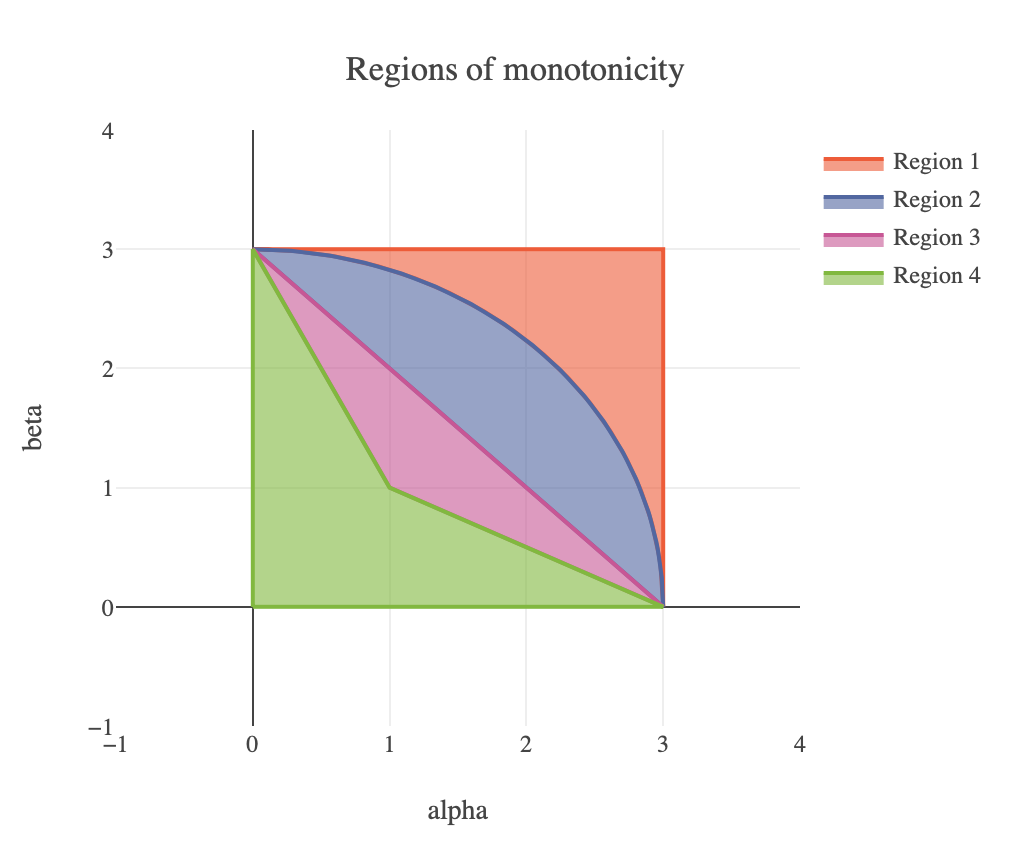
\includegraphics[scale=0.5]{Figures/splines/feasible_region.png}
  \caption{These are the feasible regions of monotonicity for cubic splines.}
  \label{fig:feasible_region}
\end{figure}

The actual region of monotonicity for a cubic polynomial is larger, but projection of $(\alpha, \beta)$ into one of these regions ensures that monotonicity will be achieved and not violated for neighboring regions. The user must decide which region is most suitable to project $(\alpha, \beta)$ onto, Fritsch and Carlson recommend using region 2.

This theoretical work has been extended in \cite{ulrich1994positivity,hess1994positive} to monotone quintic polynomials, but no mathematical software has been produced accordingly. That is where this proposed work comes in.


\section{Achieved Progress}

To expand my own understanding of the current state-of-the-art method for constructing a monotone spline interpolant, I \href{https://github.com/tchlux/VarSys/blob/master/Disseration/cubic.py}{fully implemented} the algorithm described in \cite{fritsch1980monotone} in Python. This code can be used to generate monotone cubic spline fits to data and allows for the user specification of a method((the means by which monotonicity is enforced)) and derivatives at any of the knots or endpoints. Clearly this code is not optimized for numerical robustness, nor speed, but it serves as a portable demonstration and educational tool.

Here we can see the recommended method of projection for moving cubic polynomials into the region of monotonicity.

\begin{figure}[htb]
  \centering
  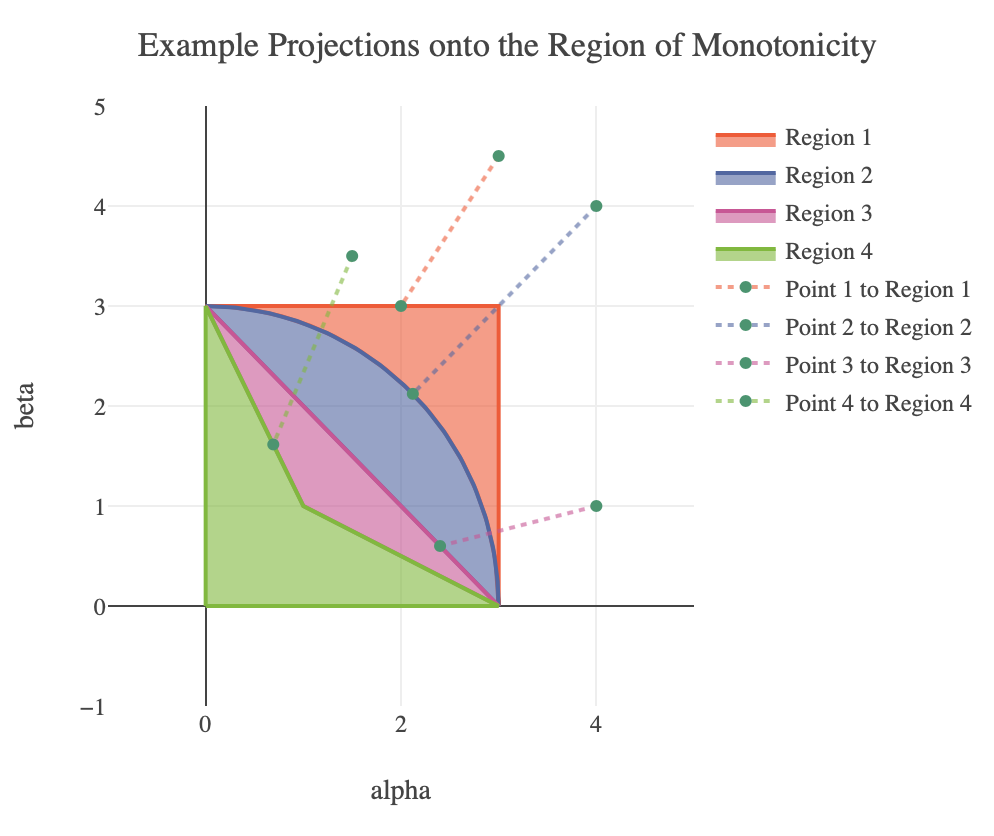
\includegraphics[scale=0.5]{Figures/splines/demo_projection.png}
  \caption{A demonstration of projection onto the feasible region for cubic splines.}
  \label{fig:demo_projection}
\end{figure}

The resulting interpolating spline is $C^1$ and has a \textit{smooth} appearance, here is a demonstration when using Region 2.

\begin{figure}[htb]
  \centering
  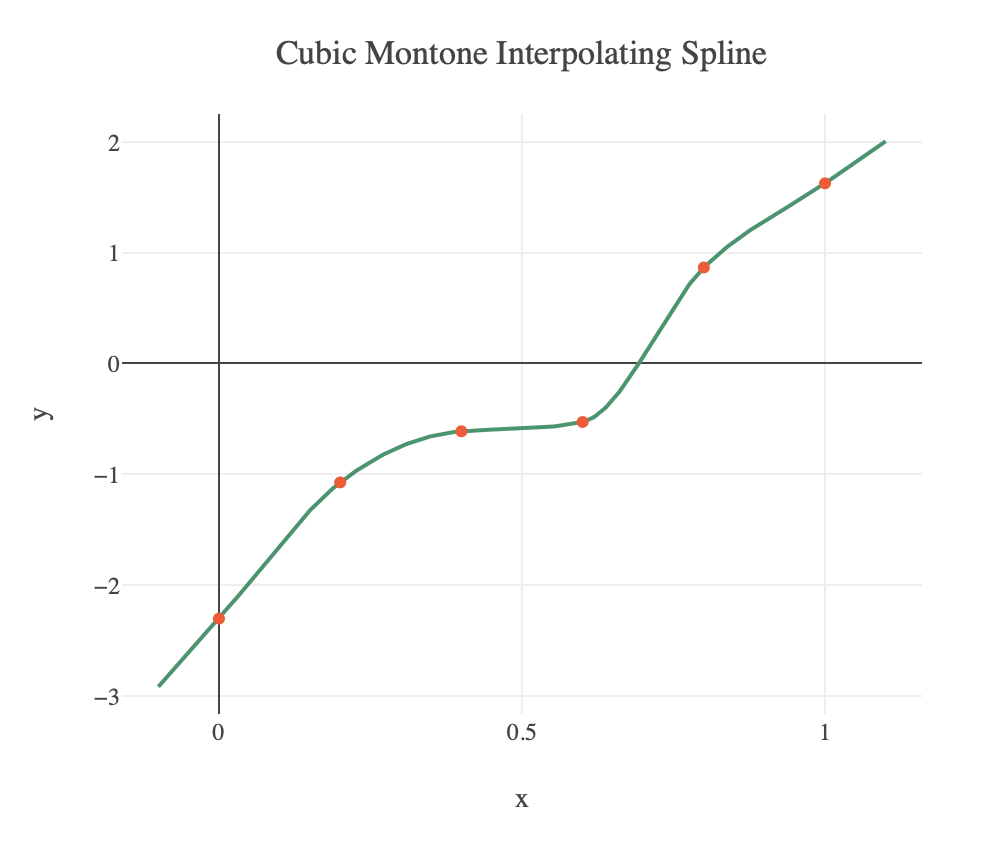
\includegraphics[scale=0.5]{Figures/splines/demo_fit.png}
  \caption{A demonstration fit with a cubic spline.}
  \label{fig:demo_fit}
\end{figure}

And the derivative of the above spline is continuous.

\begin{figure}[htb]
  \centering
  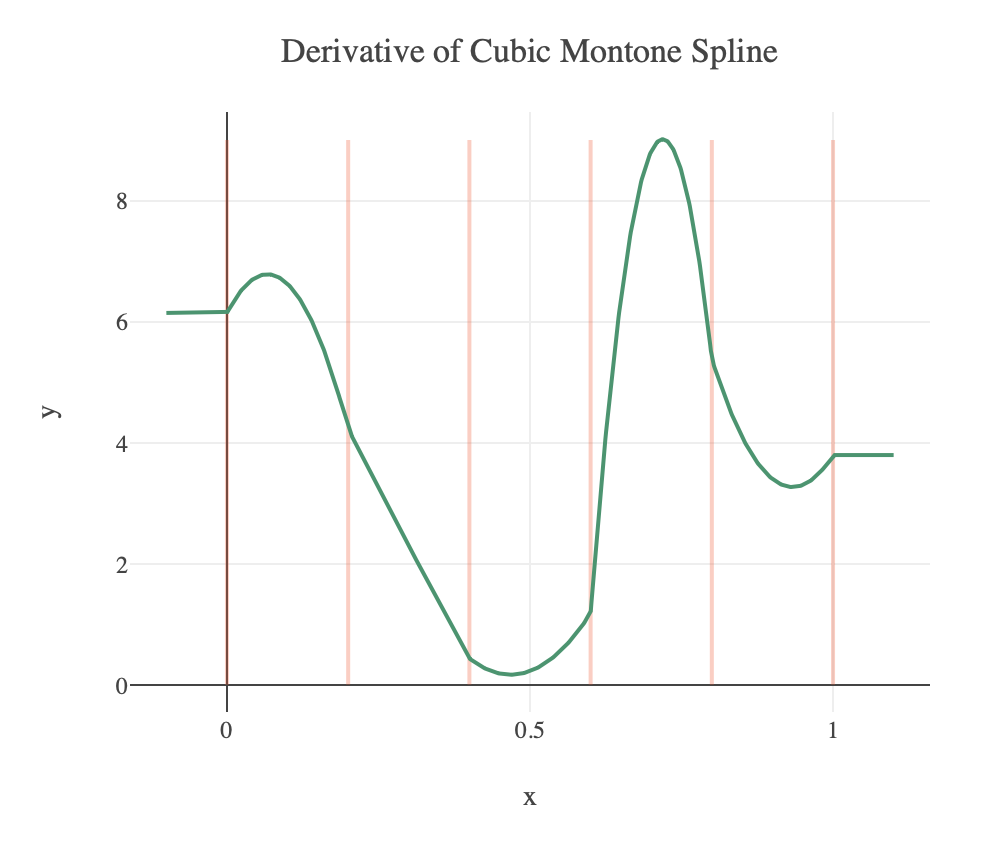
\includegraphics[scale=0.5]{./Figures/splines/demo_fit_deriv.png}
  \caption{The derivative of Figure \ref{fig:demo_projection}.}
  \label{fig:demo_fit_deriv}
\end{figure}

\section{Research Goal}

{\centering \textbf{Produce numerically robust software that computes monotone quintic interpolating splines given data.}}

\section{Timeline}

The projected research timeline is shown in Table \ref{tab:timeline}. It is expected that a significant number of \textit{unpredictable changes} will occur as the code develops and the research progresses. I will update all committee members when appropriate.

\begin{table}
  \centering
  \renewcommand{\arraystretch}{1.2}
  \begin{tabular}{l l}
    \textbf{Date} & \textbf{Milestone} \\ \hline
    \textit{June 2019} & Implementation of monotone quintic polynomial \textit{interpolant}. \\
    \textit{August 2019} & Implementation of monotone quintic polynomial \textit{spline}. \\
    \textit{October 2019} & First draft of TOMS paper on algorithm. \\
    \textit{December 2019} & Research Defense of work. \\
    \textit{March 2020} & Submission of TOMS paper and code. \\
    \textit{April 2020} & Final Defense of Ph.D.
  \end{tabular}
  \caption{This table depicts my expected timeline going forward. For details on when I achieved previous milestones, please contact me and I can provide the list. I refrained from including it here for brevity.}
  \label{tab:timeline}
\end{table}

\section{Final Remarks}

This project has the potential to be very widely utilized. As described earlier, many statistical applications could greatly benefit from having a $C^2$ approximation to CDFs, because the resulting PDF will be both aesthetically pleasing and more accurate for continuous distributions.

